%        File: arfc-beamer.tex
%     Created: Sun May 5 10:00 PM 2013 C


%\documentclass[11pt,handout]{beamer}
\documentclass[9pt]{beamer}
\usetheme[white]{Illinois}
%\title[short title]{long title}
\title[Research Summary]{Research Activities in the ARFC Group}
%\subtitle[short subtitle]{long subtitle}
\subtitle[Brief Summary]{A Brief Summary}
%\author[short name]{long name}
\author[ARFC]{Advanced Reactors and Fuel Cycles Group}
%\date[short date]{long date}
\date[09.05.2019]{September 5, 2019}
%\institution[short name]{long name}
\institute[UIUC]{University of Illinois at Urbana-Champaign}

%\usepackage{bbding}
\usepackage{amsfonts}
\usepackage{amsmath}
\usepackage{xspace}
\usepackage{graphicx}
\usepackage{subfigure}
\usepackage{booktabs} % nice rules for tables
\usepackage{microtype} % if using PDF
\usepackage{bigints}
\usepackage{tikz}
\usetikzlibrary{positioning, arrows, decorations, shapes}
\definecolor{illiniblue}{HTML}{B1C6E2}
\definecolor{illiniorange}{HTML}{f8c2a2}
\usetikzlibrary{shapes.geometric, arrows}
\tikzstyle{oblock} = [rectangle, draw, fill=illiniorange,
text width=15em, text centered, rounded corners, minimum height=4em]
\tikzstyle{bblock} = [rectangle, draw, fill=illiniblue,
text width=15em, text centered, rounded corners, minimum height=4em]
\tikzstyle{arrow} = [thick,->,>=stealth]

\usepackage{tabularx}
\newcolumntype{b}{>{\hsize=1.0\hsize}X}
\newcolumntype{s}{>{\hsize=.5\hsize}X}
\newcolumntype{m}{>{\hsize=.75\hsize}X}
\newcolumntype{x}{>{\hsize=.25\hsize}X}
\newcolumntype{L}{>{\raggedright\arraybackslash}X}
\newcolumntype{R}{>{\raggedleft\arraybackslash}X}
\def\arraystretch{1}

\newcommand{\Cyclus}{\textsc{Cyclus}\xspace}%
\newcommand{\Cycamore}{\textsc{Cycamore}\xspace}%
\newcommand{\deploy}{\texttt{d3ploy}\xspace}%
\newcommand{\units}[1] {\:\text{#1}}%
\newcommand{\SN}{S$_N$}%{S$_\text{N}$}%{$S_N$}%
\DeclareMathOperator{\erf}{erf}
%I need some complimentary error funcitons...
\DeclareMathOperator{\erfc}{erfc}
%Those icons in the references are terrible looking
\setbeamertemplate{bibliography item}[text]

\usepackage{multirow}
\usepackage{graphicx,subfigure}

%%%% Acronym support

\usepackage[acronym,toc]{glossaries}
%\newacronym{<++>}{<++>}{<++>}
\newacronym[longplural={metric tons of heavy metal}]{MTHM}{MTHM}{metric ton of heavy metal}
\newacronym{ABM}{ABM}{agent-based modeling}
\newacronym{ACDIS}{ACDIS}{Program in Arms Control \& Domestic and International Security}
\newacronym{AHTR}{AHTR}{Advanced High Temperature Reactor}
\newacronym{ANDRA}{ANDRA}{Agence Nationale pour la gestion des D\'echets RAdioactifs, the French National Agency for Radioactive Waste Management}
\newacronym{ANL}{ANL}{Argonne National Laboratory}
\newacronym{API}{API}{application programming interface}
\newacronym{ARE}{ARE}{Aircraft Reactor Experiment}
\newacronym{ARFC}{ARFC}{Advanced Reactors and Fuel Cycles}
\newacronym{ASME}{ASME}{American Society of Mechanical Engineers}
\newacronym{ATWS}{ATWS}{Anticipated Transient Without Scram}
\newacronym{BDBE}{BDBE}{Beyond Design Basis Event}
\newacronym{BIDS}{BIDS}{Berkeley Institute for Data Science}
\newacronym{CAFCA}{CAFCA}{ Code for Advanced Fuel Cycles Assessment }
\newacronym{CDTN}{CDTN}{Centro de Desenvolvimento da Tecnologia Nuclear}
\newacronym{CEA}{CEA}{Commissariat \`a l'\'Energie Atomique et aux \'Energies Alternatives}
\newacronym{CI}{CI}{continuous integration}
\newacronym{CNEN}{CNEN}{Comiss\~{a}o Nacional de Energia Nuclear}
\newacronym{CNERG}{CNERG}{Computational Nuclear Engineering Research Group}
\newacronym{COSI}{COSI}{Commelini-Sicard}
\newacronym{COTS}{COTS}{commercial, off-the-shelf}
\newacronym{CSNF}{CSNF}{commercial spent nuclear fuel}
\newacronym{CTAH}{CTAHs}{Coiled Tube Air Heaters}
\newacronym{CUBIT}{CUBIT}{CUBIT Geometry and Mesh Generation Toolkit}
\newacronym{CURIE}{CURIE}{Centralized Used Fuel Resource for Information Exchange}
\newacronym{DAG}{DAG}{directed acyclic graph}
\newacronym{DANESS}{DANESS}{Dynamic Analysis of Nuclear Energy System Strategies}
\newacronym{DBE}{DBE}{Design Basis Event}
\newacronym{DESAE}{DESAE}{Dynamic Analysis of Nuclear Energy Systems Strategies}
\newacronym{DHS}{DHS}{Department of Homeland Security}
\newacronym{DOE}{DOE}{Department of Energy}
\newacronym{DRACS}{DRACS}{Direct Reactor Auxiliary Cooling System}
\newacronym{DRE}{DRE}{dynamic resource exchange}
\newacronym{DSNF}{DSNF}{DOE spent nuclear fuel}
\newacronym{DYMOND}{DYMOND}{Dynamic Model of Nuclear Development }
\newacronym{EBS}{EBS}{Engineered Barrier System}
\newacronym{EDZ}{EDZ}{Excavation Disturbed Zone}
\newacronym{EIA}{EIA}{U.S. Energy Information Administration}
\newacronym{EPA}{EPA}{Environmental Protection Agency}
\newacronym{EP}{EP}{Engineering Physics}
\newacronym{FCO}{FCO}{Fuel Cycle Options}
\newacronym{FCT}{FCT}{Fuel Cycle Technology}
\newacronym{FEHM}{FEHM}{Finite Element Heat and Mass Transfer}
\newacronym{FEPs}{FEPs}{Features, Events, and Processes}
\newacronym{FHR}{FHR}{Fluoride-Salt-Cooled High-Temperature Reactor}
\newacronym{FLiBe}{FLiBe}{Fluoride-Lithium-Beryllium}
\newacronym{GDSE}{GDSE}{Generic Disposal System Environment}
\newacronym{GDSM}{GDSM}{Generic Disposal System Model}
\newacronym{GENIUSv1}{GENIUSv1}{Global Evaluation of Nuclear Infrastructure Utilization Scenarios, Version 1}
\newacronym{GENIUSv2}{GENIUSv2}{Global Evaluation of Nuclear Infrastructure Utilization Scenarios, Version 2}
\newacronym{GENIUS}{GENIUS}{Global Evaluation of Nuclear Infrastructure Utilization Scenarios}
\newacronym{GPAM}{GPAM}{Generic Performance Assessment Model}
\newacronym{GRSAC}{GRSAC}{Graphite Reactor Severe Accident Code}
\newacronym{GUI}{GUI}{graphical user interface}
\newacronym{HLW}{HLW}{high level waste}
\newacronym{HPC}{HPC}{high-performance computing}
\newacronym{HTC}{HTC}{high-throughput computing}
\newacronym{HTGR}{HTGR}{High Temperature Gas-Cooled Reactor}
\newacronym{IAEA}{IAEA}{International Atomic Energy Agency}
\newacronym{IEMA}{IEMA}{Illinois Emergency Mangament Agency}
\newacronym{INL}{INL}{Idaho National Laboratory}
\newacronym{IPRR1}{IRP-R1}{Instituto de Pesquisas Radioativas Reator 1}
\newacronym{IRP}{IRP}{Integrated Research Project}
\newacronym{ISFSI}{ISFSI}{Independent Spent Fuel Storage Installation}
\newacronym{ISRG}{ISRG}{Independent Student Research Group}
\newacronym{JFNK}{JFNK}{Jacobian-Free Newton Krylov}
\newacronym{LANL}{LANL}{Los Alamos National Laboratory}
\newacronym{LBNL}{LBNL}{Lawrence Berkeley National Laboratory}
\newacronym{LCOE}{LCOE}{levelized cost of electricity}
\newacronym{LDRD}{LDRD}{laboratory directed research and development}
\newacronym{LFR}{LFR}{Lead-Cooled Fast Reactor}
\newacronym{LLNL}{LLNL}{Lawrence Livermore National Laboratory}
\newacronym{LMFBR}{LMFBR}{Liquid Metal Fast Breeder Reactor}
\newacronym{LOFC}{LOFC}{Loss of Forced Cooling}
\newacronym{LOHS}{LOHS}{Loss of Heat Sink}
\newacronym{LOLA}{LOLA}{Loss of Large Area}
\newacronym{LP}{LP}{linear program}
\newacronym{LWR}{LWR}{Light Water Reactor}
\newacronym{MA}{MA}{minor actinide}
\newacronym{MCNP}{MCNP}{Monte Carlo N-Particle code}
\newacronym{MILP}{MILP}{mixed-integer linear program}
\newacronym{MIT}{MIT}{the Massachusetts Institute of Technology}
\newacronym{MOAB}{MOAB}{Mesh-Oriented datABase}
\newacronym{MOOSE}{MOOSE}{Multiphysics Object-Oriented Simulation Environment}
\newacronym{MOX}{MOX}{mixed oxide}
\newacronym{MSBR}{MSBR}{Molten Salt Breeder Reactor}
\newacronym{MSRE}{MSRE}{Molten Salt Reactor Experiment}
\newacronym{MSR}{MSR}{Molten Salt Reactor}
\newacronym{NAGRA}{NAGRA}{National Cooperative for the Disposal of Radioactive Waste}
\newacronym{NEAMS}{NEAMS}{Nuclear Engineering Advanced Modeling and Simulation}
\newacronym{NEUP}{NEUP}{Nuclear Energy University Programs}
\newacronym{NFCSim}{NFCSim}{Nuclear Fuel Cycle Simulator}
\newacronym{NGNP}{NGNP}{Next Generation Nuclear Plant}
\newacronym{NMWPC}{NMWPC}{Nuclear MW Per Capita}
\newacronym{NNSA}{NNSA}{National Nuclear Security Administration}
\newacronym{NPRE}{NPRE}{Department of Nuclear, Plasma, and Radiological Engineering}
\newacronym{NQA1}{NQA-1}{Nuclear Quality Assurance - 1}
\newacronym{NRC}{NRC}{Nuclear Regulatory Commission}
\newacronym{NSF}{NSF}{National Science Foundation}
\newacronym{NSSC}{NSSC}{Nuclear Science and Security Consortium}
\newacronym{NUWASTE}{NUWASTE}{Nuclear Waste Assessment System for Technical Evaluation}
\newacronym{NWF}{NWF}{Nuclear Waste Fund}
\newacronym{NWTRB}{NWTRB}{Nuclear Waste Technical Review Board}
\newacronym{OCRWM}{OCRWM}{Office of Civilian Radioactive Waste Management}
\newacronym{ORION}{ORION}{ORION}
\newacronym{ORNL}{ORNL}{Oak Ridge National Laboratory}
\newacronym{PARCS}{PARCS}{Purdue Advanced Reactor Core Simulator}
\newacronym{PBAHTR}{PB-AHTR}{Pebble Bed Advanced High Temperature Reactor}
\newacronym{PBFHR}{PB-FHR}{Pebble-Bed Fluoride-Salt-Cooled High-Temperature Reactor}
\newacronym{PEI}{PEI}{Peak Environmental Impact}
\newacronym{PH}{PRONGHORN}{PRONGHORN}
\newacronym{PRKE}{PRKE}{Point Reactor Kinetics Equations}
\newacronym{PSPG}{PSPG}{Pressure-Stabilizing/Petrov-Galerkin}
\newacronym{PWAR}{PWAR}{Pratt and Whitney Aircraft Reactor}
\newacronym{PWR}{PWR}{Pressurized Water Reactor}
\newacronym{PyNE}{PyNE}{Python toolkit for Nuclear Engineering}
\newacronym{PyRK}{PyRK}{Python for Reactor Kinetics}
\newacronym{QA}{QA}{quality assurance}
\newacronym{RDD}{RD\&D}{Research Development and Demonstration}
\newacronym{RD}{R\&D}{Research and Development}
\newacronym{RELAP}{RELAP}{Reactor Excursion and Leak Analysis Program}
\newacronym{RIA}{RIA}{Reactivity Insertion Accident}
\newacronym{RIF}{RIF}{Region-Institution-Facility}
\newacronym{SFR}{SFR}{Sodium-Cooled Fast Reactor}
\newacronym{SINDAG}{SINDA{\textbackslash}G}{Systems Improved Numerical Differencing Analyzer $\backslash$ Gaski}
\newacronym{SKB}{SKB}{Svensk K\"{a}rnbr\"{a}nslehantering AB}
\newacronym{SNF}{SNF}{spent nuclear fuel}
\newacronym{SNL}{SNL}{Sandia National Laboratory}
\newacronym{STC}{STC}{specific temperature change}
\newacronym{SUPG}{SUPG}{Streamline-Upwind/Petrov-Galerkin}
\newacronym{SWF}{SWF}{Separations and Waste Forms}
\newacronym{SWU}{SWU}{Separative Work Unit}
\newacronym{TRIGA}{TRIGA}{Training Research Isotope General Atomic}
\newacronym{TRISO}{TRISO}{Tristructural Isotropic}
\newacronym{TSM}{TSM}{Total System Model}
\newacronym{TSPA}{TSPA}{Total System Performance Assessment for the Yucca Mountain License Application}
\newacronym{ThOX}{ThOX}{thorium oxide}
\newacronym{UFD}{UFD}{Used Fuel Disposition}
\newacronym{UML}{UML}{Unified Modeling Language}
\newacronym{UOX}{UOX}{uranium oxide}
\newacronym{UQ}{UQ}{uncertainty quantification}
\newacronym{US}{US}{United States}
\newacronym{UW}{UW}{University of Wisconsin}
\newacronym{VISION}{VISION}{the Verifiable Fuel Cycle Simulation Model}
\newacronym{VV}{V\&V}{verification and validation}
\newacronym{WIPP}{WIPP}{Waste Isolation Pilot Plant}
\newacronym{YMR}{YMR}{Yucca Mountain Repository Site}


\makeglossaries

%try to get rid of header on title page\dots
\makeatletter
    \newenvironment{withoutheadline}{
        \setbeamertemplate{headline}[default]
        \def\beamer@entrycode{\vspace*{-\headheight}}
    }{}
\makeatother

\makeatother
\setbeamertemplate{footline}
{
  \leavevmode%
  \hbox{%
    \rightline{\insertframenumber{} / \inserttotalframenumber\hspace*{1ex}}
  }%
  \vskip0pt%
}
\makeatletter
\begin{document}
%%%%%%%%%%%%%%%%%%%%%%%%%%%%%%%%%%%%%%%%%%%%%%%%%%%%%%%%%%%%%
%% From uw-beamer Here's a handy bit of code to place at 
%% the beginning of your presentation (after \begin{document}):
\newcommand*{\alphabet}{ABCDEFGHIJKLMNOPQRSTUVWXYZabcdefghijklmnopqrstuvwxyz}
\newlength{\highlightheight}
\newlength{\highlightdepth}
\newlength{\highlightmargin}
\setlength{\highlightmargin}{2pt}
\settoheight{\highlightheight}{\alphabet}
\settodepth{\highlightdepth}{\alphabet}
\addtolength{\highlightheight}{\highlightmargin}
\addtolength{\highlightdepth}{\highlightmargin}
\addtolength{\highlightheight}{\highlightdepth}
\newcommand*{\Highlight}{\rlap{\textcolor{HighlightBackground}{\rule[-\highlightdepth]{\linewidth}{\highlightheight}}}}
%%%%%%%%%%%%%%%%%%%%%%%%%%%%%%%%%%%%%%%%%%%%%%%%%%%%%%%%%%%%%
%%--------------------------------%%
\begin{withoutheadline}
\frame{
  \titlepage
}
\end{withoutheadline}

%%--------------------------------%%
\AtBeginSection[]{
\begin{frame}
  \frametitle{Outline}
  \tableofcontents[currentsection]
\end{frame}
}

\section{Pyre}
\begin{frame}
  \frametitle{Motivation/Goals}
  	\textbf{Motivation}
        \begin{itemize}
                \item Safeguard by design
                \item Model diversion inside facilities
                \item transition from LWR to SFR
        \end{itemize}
    \textbf{Goals}
    	\begin{itemize}
    		\item Detect diversion using signatures and observables.
    		\item Optimum detector and inspection locations in pyroprocessing
    		\item Characterize detection sensitivities and false positive rates
    	\end{itemize}
\end{frame}

\begin{frame}
	\frametitle{PyRe Archetype}
	\begin{columns}
		\column[t]{5cm}
		\begin{itemize}
			\item Facility containing multiple sub-processes:
			\begin{itemize}
				\item Separately handled.
				\item Independent transactions, possibility of diversion.
			\end{itemize}
			\item Operation setting impact efficiency.
			\item Generic facility:
			\begin{itemize}
				\item Multiple types of pyro plants.
				\item LWR vs SFR.
			\end{itemize}
		\end{itemize}
		\column[t]{6cm}
		\begin{figure}
			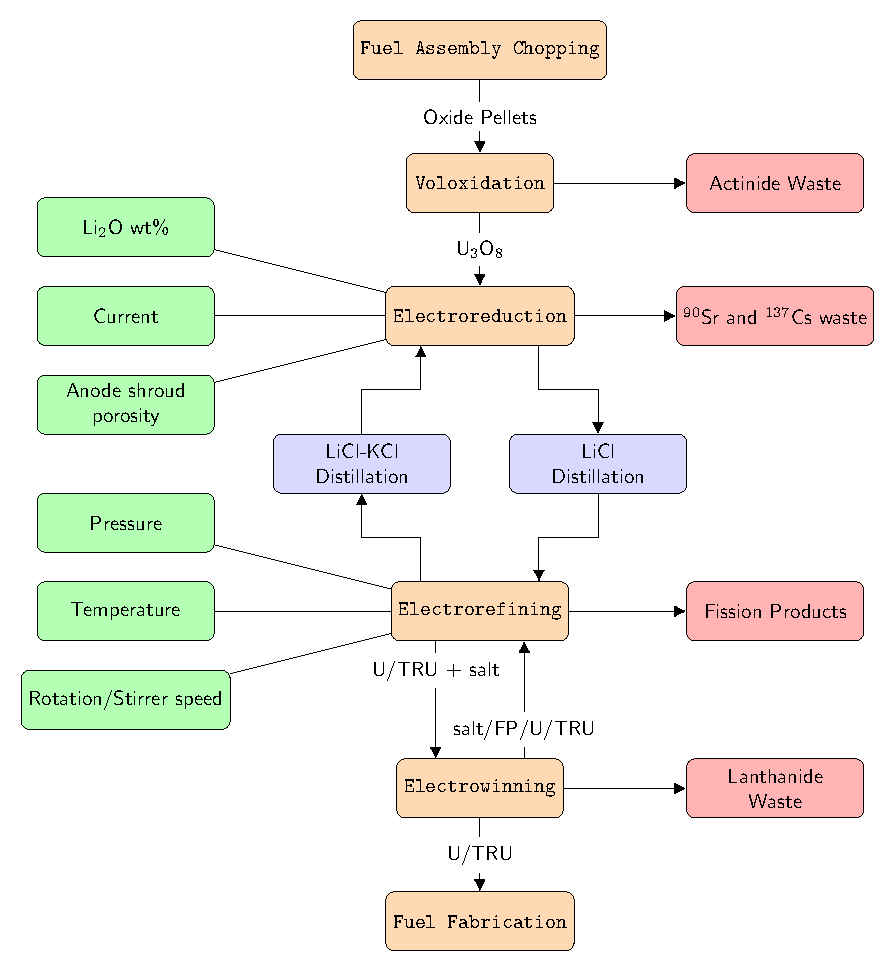
\includegraphics[width=\linewidth]{./images/westphal-pyre.pdf}
			\caption{PyRe flow diagram for LWR waste configuration.}
			\label{fig:pyre}
		\end{figure}
	\end{columns}
\end{frame}

\begin{frame}
\frametitle{Pyre - Diversion Options}
Material diversion occurs in two different modes: \textbf{nefarious} or \textbf{operator}.
\begin{itemize}
	\item \textbf{Nefarious Diversion} imagines diversion by a single bad actor with facility access.
	\item \textbf{Operator Diversion} imagines undeclared production.
\end{itemize}
\begin{figure}
	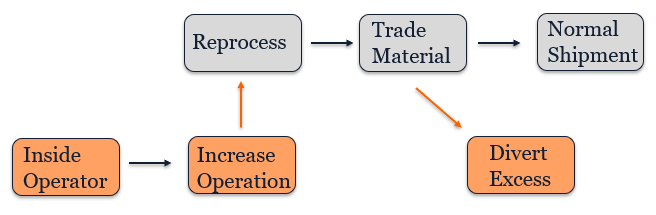
\includegraphics[width=0.7\linewidth]{./images/westphal-diversion}
	\caption{Operator vs nefarious diversion.}
	\label{fig:diversion}
\end{figure}
\end{frame}

\begin{frame}
	\frametitle{Diverter Class}
	\begin{columns}
		\column[t]{5cm}
		Inputs:
		\begin{itemize}
			\item Location
			\begin{itemize}
				\item Sub-process
				\item Operation Setting
			\end{itemize}
			\item Quantity
			\item Frequency
			\item Number of Diversions
		\end{itemize}
		\begin{block}{Purpose}
			The goal of a separate diverter class is to allow this method to be used by facilities other
			than pyre through a toolkit.
		\end{block}
		\column[t]{6cm}
		\begin{figure}
			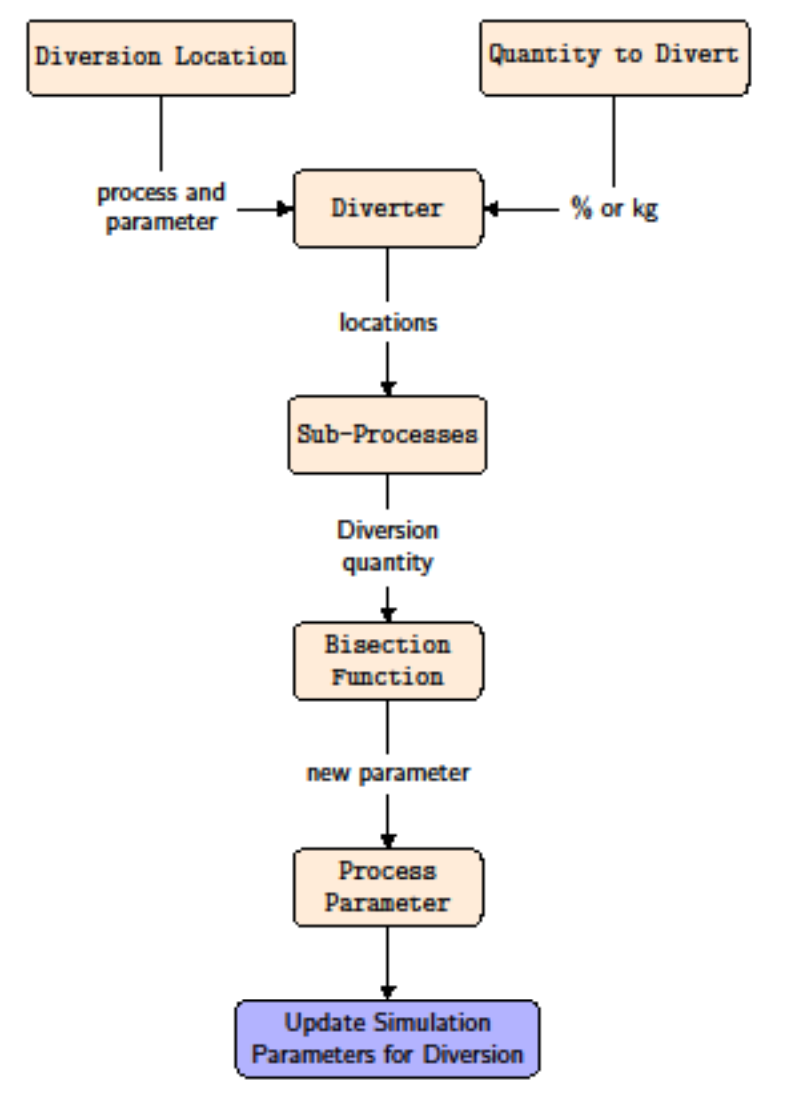
\includegraphics[width=0.8\linewidth]{images/diverter}
			\label{fig:diverter}
		\end{figure}
	\end{columns}
\end{frame}

\begin{frame}
\frametitle{Diversion Detection}
\begin{columns}
	\column[t]{5cm}
	\begin{block}{Diversion Detection}
		Material transactions are no longer a reliable method. Instead we use
		signatures and observables:
		\begin{itemize}
			\item Temperature, power draw, etc.
		\end{itemize}
		A Cumulative Sum change algorithm is used to detect any significant changes.
	\end{block}
	\column[t]{6cm}
	\begin{figure}
		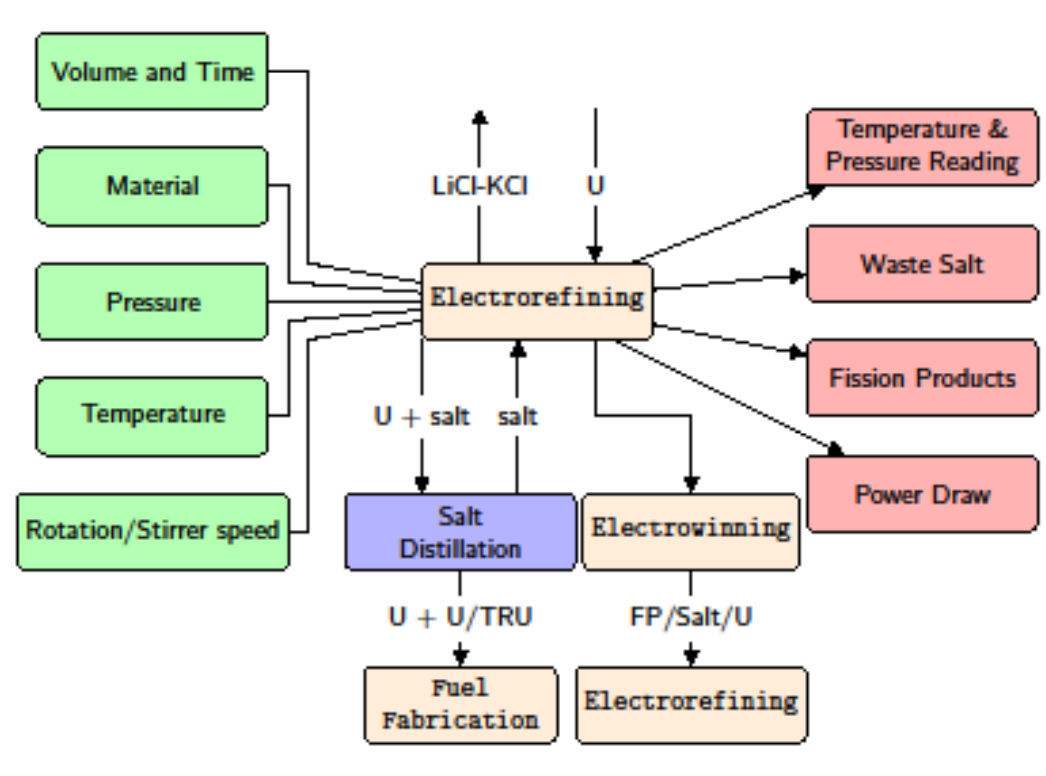
\includegraphics[width=\linewidth]{images/refining}
	\end{figure}
\end{columns}
\end{frame}

\begin{frame}
\frametitle{Transition Scenario}
A main attraction of pyroprocessing is the ability to handle LWR and
SFR waste.
\begin{itemize}
	\item To verify this capability in PyRe, we ran an EG01 – EG24 transition
	scenario.
	\item We want to observe the following:
	\begin{itemize}
		\item Appropriate deploying of PyRe
		\item Ability to meet demand of new SFRs
		\item Diversion capabilities
		\item Accurate transition from UOX to SFR fuels
	\end{itemize}
\end{itemize}
\end{frame}

\begin{frame}
\frametitle{Transition Scenario - Results}
\begin{figure}
	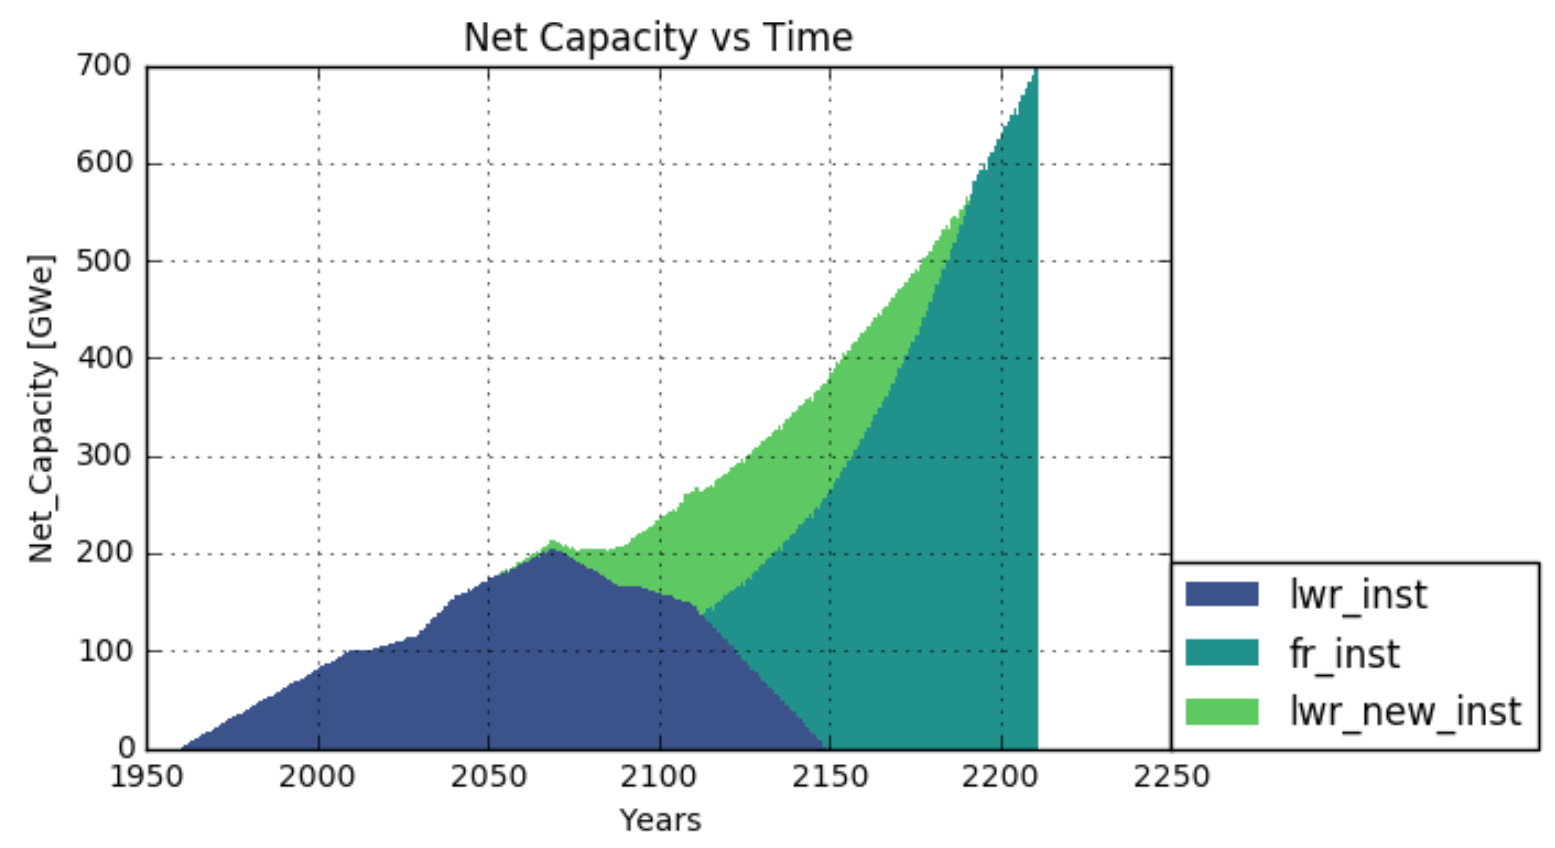
\includegraphics[width=\linewidth]{images/netcap}
\end{figure}
\end{frame}

\begin{frame}
\frametitle{Diversion Settings}
\begin{columns}
	\column[t]{4cm}
	Two Pyre prototypes:
	\begin{itemize}
		\item LWR vs SFR
	\end{itemize}
	LWR Pyre:
	\begin{itemize}
		\item Fewer diversions
		\item More material per instance
		\item Less frequent
	\end{itemize}
	SFR Pyre:
	\begin{itemize}
		\item Frequent diversion
		\item Small quantities
	\end{itemize}
	\column[t]{7cm}
	\begin{figure}
		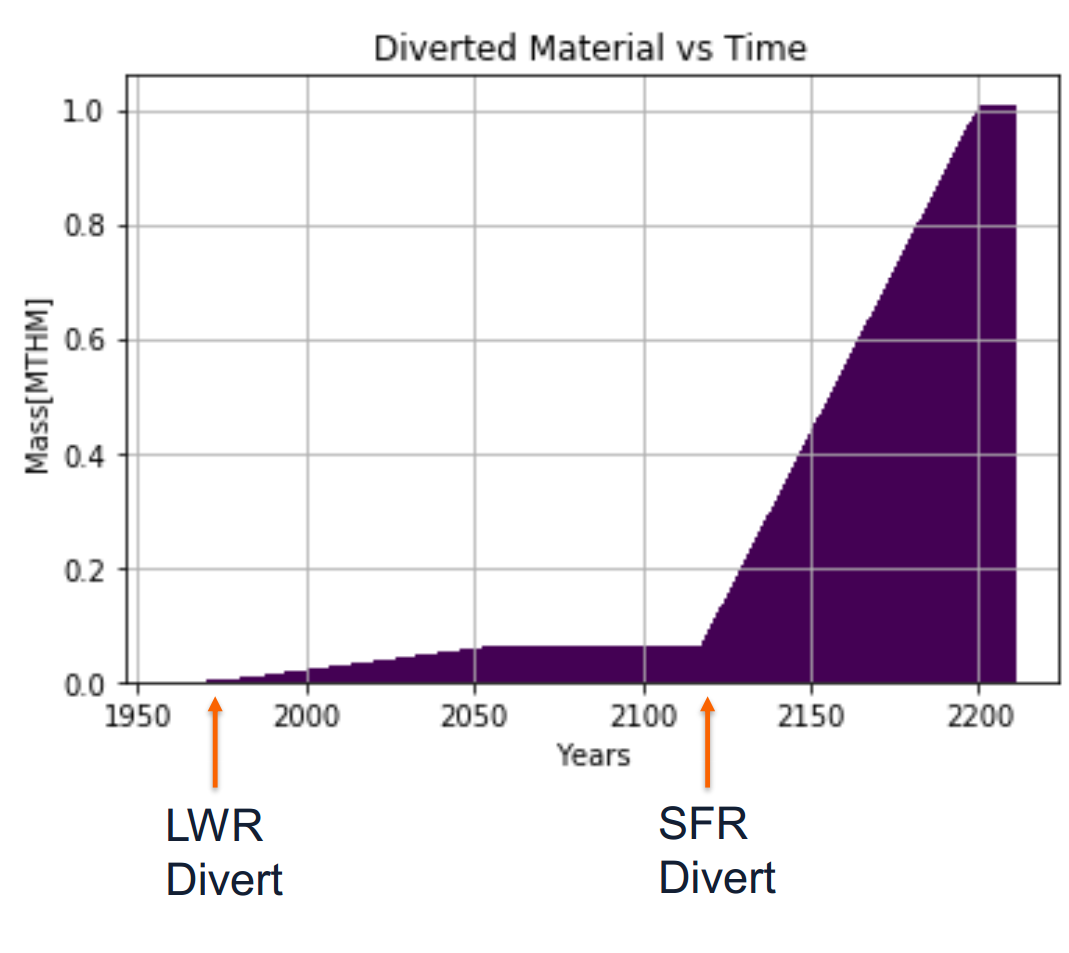
\includegraphics[width=\linewidth]{images/divertmat}
	\end{figure}
\end{columns}
\end{frame}

\begin{frame}
\frametitle{Transition Scenario - Utilization}
\begin{figure}
	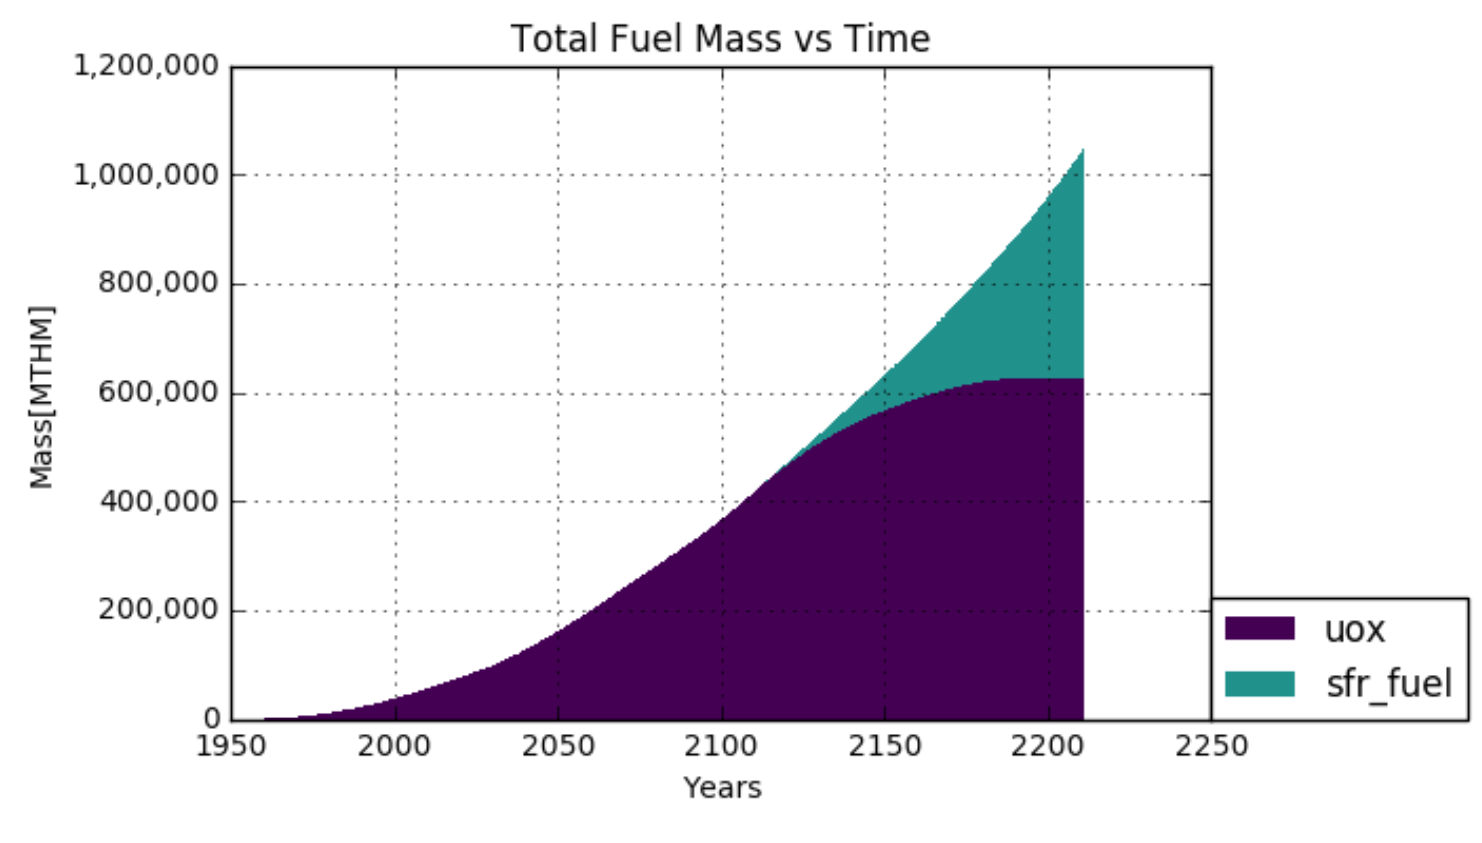
\includegraphics[width=\linewidth]{images/fuelmass}
\end{figure}
\end{frame}

\begin{frame}
\frametitle{Conclusions}
We have developed a customizable method of diverting material
from inside Cyclus facilities.
\begin{itemize}
	\item Preliminary work has been done on the detection of two
	different types of diversion: Nefarious and Operator
\end{itemize}
PyRe was demonstrated to function as both LWR and SFR
reprocessing method
\begin{itemize}
	\item Generic facility capable of modeling multiple facility layouts
\end{itemize}
\end{frame}
\section{DDCA}
\begin{frame}
        \frametitle{DDCA Overview}
        \begin{itemize}
                  \setlength{\itemindent}{1cm}
                \item[\textbf{Title:}] Demand-Driven Cycamore Archetypes 
                \item[\textbf{PI:}] Anthony Scopatz, University of South 
                        Carolina\footnote{Anthony departed academia in year 2 
                        of the project. The PIship was transferred to Travis 
                        Knight at USC}
                \item[\textbf{Co-PI:}] Kathryn Huff, University of Illinois at 
                        Urbana-Champaign
                \item[\textbf{Start:}] October, 2016
                \item[\textbf{End:}] October, 2017
                \item[\textbf{Objectives:}] Develop an in situ demand 
                        driven development schedule calculation through 
                        non-optimizing, deterministic-optimizing, and 
                        stochastic-optimizing algorithms as Cyclus archetypes. 
                        Demonstrate these new archetypes in program-supporting 
                        fuel cycle scenarios.
        \end{itemize}
\end{frame}


\begin{frame}
        \frametitle{Quick Statistics}
        \begin{block}{Publications Affiliated with this Work}
                \begin{itemize}
                  \setlength{\itemindent}{3cm}
                        \item[\textbf{Journal Articles}] 3 (2 upcoming)
                        \item[\textbf{Full Conference Papers}] 3 (2 upcoming) 
                        \item[\textbf{Conference Summaries}] 7
                        \item[\textbf{Technical Reports}] 2 (1 upcoming)
                        \item[\textbf{Theses}] 1MS (2 upcoming)
                \end{itemize}
        \end{block}

                \begin{block}{Students Supported}
                        The funding supported graduate students and 
                        occasional undergraduates at UIUC.
                        \textbf{Jin Whan Bae} recieved his MS and is now at 
                        ORNL purusing Cyclus usability.
                        \textbf{Gwendolyn Chee} is writing an MS thesis related 
                        to this work and related work conducted at ANL with Bo Feng.
                        Undergraduate \textbf{Louis Kissinger} is a 
                        baccalaureate researcher this year in MCS at ANL.
                        Others include \textbf{Roberto Fairhurst}, \textbf{Gyu 
                        Tae Park}, \textbf{Snehal Chandan}, and \textbf{Aditya 
                        Bhosale}.
                \end{block}
\end{frame}

\begin{frame}
  \frametitle{Motivation}
  % a comment
        \begin{block}{Main Objective}
              To improve usability of Cyclus for transition scenarios.
        \end{block}
        

        \begin{block}{Main Challenge}
              Deploying reactors to meet power demand is trivial, and existed 
                in the earliest versions of Cyclus.
              \textbf{Automated, predictive deployment and decommissioning of 
                other facilities is more complex.} These include mining, 
                milling, enrichment, fuel 
                fabrication, reprocessing, and others. 

              For example, a balanced closed fuel cycle may require ensuring 
                that there is enough fast reactor fuel for their operation and 
                may drive deployment of a fleet of light water reactors.
        \end{block}
\end{frame}

\begin{frame}
\frametitle{Goals}
\textbf{Goals of this work} 
\begin{itemize}
	\item Develop demand driven deployment capabilities in \Cyclus (\deploy)
	\item Demonstrate the use of \deploy to set up EG01-23, EG01-24, EG01-29
	EG01-30 transition scenarios with constant and linearly increasing 
	power demand curves. 
\end{itemize}

\end{frame}

\begin{frame}
\frametitle{Method}
\begin{block}{Because Cyclus is Agent-Based}
	\begin{itemize}
		\item Its regions and institutions have the agency to dynamically make and alter deployment decisions.
		\item Each agent can make their own predictions of the future based on current and past performance of the simulation.
	\end{itemize}
	
	We embedded advanced time series prediction algorithms to automatically
	deploy fuel cycle facilities for the user. This was implemented
	in \textbf{\texttt{d3ploy}}, an Institution agent.
\end{block}
\end{frame}

%\begin{frame}
%  \frametitle{Goal of the Project}
%  % a comment
%  \begin{itemize}
%    \item[$\bullet$] Three types of methods were looked at for doing the prediction.
%    \item[$\bullet$] Non-optimizing methods. These methods included moving average
%                     , autoregressive moving average (ARMA), and autoregressive
%                     heteroskidasticity (ARCH) models.
%    \item[$\bullet$] Deterministic models. These models use a methodology that will
%                     always return the same answer given a unique input. This includes
%                     Fast Fourier Transforms, Exponential Smoothing, Holt-Winters,
%                     Polynomial regression.
%    \item[$\bullet$] Stochastic models. With stochastic models, the output is based
%                     on randomly sampling models to determine the behavior of the
%                     next time step. The method implimented here is a machine learning
%                     seasonal method.
%   \end{itemize}
%\end{frame}
%

\begin{frame}
\frametitle{Motivation}

\textbf{Gap in capability: User must define when support facilities are deployed}

\begin{figure}[htbp!]
\begin{center}
	
\includegraphics[width=0.8\textwidth]{images/user-deploy}
\end{center}
\caption{User defined Deployment Scheme }
\end{figure}

\textbf{Bridging the gap: Developed demand-driven deployment capability in \Cyclus. This capability is named \deploy.}

\begin{figure}[htbp!]
\begin{center}
	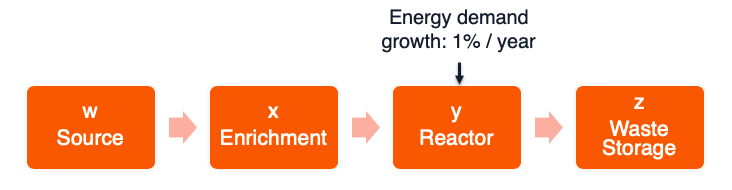
\includegraphics[width=0.8\textwidth]{images/auto-deploy}
\end{center}
\caption{Demand Driven Deployment Scheme}
\end{figure}

\end{frame}

\begin{frame}
\frametitle{\deploy Objectives}
\textbf{\deploy's Main Objective}
\vspace{0.3em}
\\
Minimize the number of time steps of undersupply or under capacity 
of power.
\vspace{1em}
\\
\textbf{\deploy's Sub-Objectives}
\begin{itemize}
	\item Minimize the number of time steps of undersupply or under capacity 
	of any commodity.
	\item Minimize excessive oversupply of all commodities  
\end{itemize} 
\end{frame}

\begin{frame}
\frametitle{\deploy Input Parameters}
\begin{table}[]
\centering
\caption{\deploy's required and optional input parameters with examples.}
\label{tab:inputs}
\footnotesize
\begin{tabularx}{\textwidth}{l|LL}
	\hline
	& \textbf{Input Parameter}                                                           & \textbf{Examples}                                                                                                          \\ \hline
	\multirow{5}{*}{\textbf{Required}} & Demand driving commodity                                                           & Power, Fuel, Plutonium, etc.                                                                                                                      \\ 
	& Demand equation                                                                    & P(t) = 10000, sin(t), 10000*t                                                                                                                 \\ \cline{2-3} 
	& Facilities it controls                                                             & Fuel Fab, LWR reactor, SFR reactor, Waste repository, etc.                                                                                                      \\ \cline{2-3} 
	& Capacities of the facilities                                                       & 3000 kg, 1000 MW, 50000 kg                                                                                                     \\ \cline{2-3} 
	& Prediction method                                                                  & \begin{tabular}[c]{@{}l@{}}Power: fast fourier transform\\ Fuel: moving average\\ Spent fuel: moving average\end{tabular} \\ \cline{2-3} 
	& Deployment driven by & Installed Capacity/Supply                                                                                                                    \\ \hline
	\multirow{4}{*}{\textbf{Optional}} & Supply/Capacity Buffer type                                                                        & Absolute                                                                                                                  \\ \cline{2-3} 
	& Supply/Capacity Buffer size                                                                        & \begin{tabular}[c]{@{}l@{}}Power: 3000 MW\\ Fuel: 0 kg \\ Spent fuel: 0 kg\end{tabular}                                   \\ \cline{2-3} 
	& Facility preferences                                                               & \begin{tabular}[c]{@{}l@{}}LWR reactor = 100-t\\ SFR reactor = t-100 \end{tabular}          \\ \cline{2-3} 
	& Facility constraint                                                              & SFR reactor constraint = 5000kg of Pu            \\ \hline	
\end{tabularx}
\end{table}
\end{frame}

\begin{frame}
\frametitle{\deploy logic flow}
\begin{columns}
\column[t]{8cm}
\begin{figure}[]
\centering
\resizebox{0.7\textwidth} {0.45\height}{
	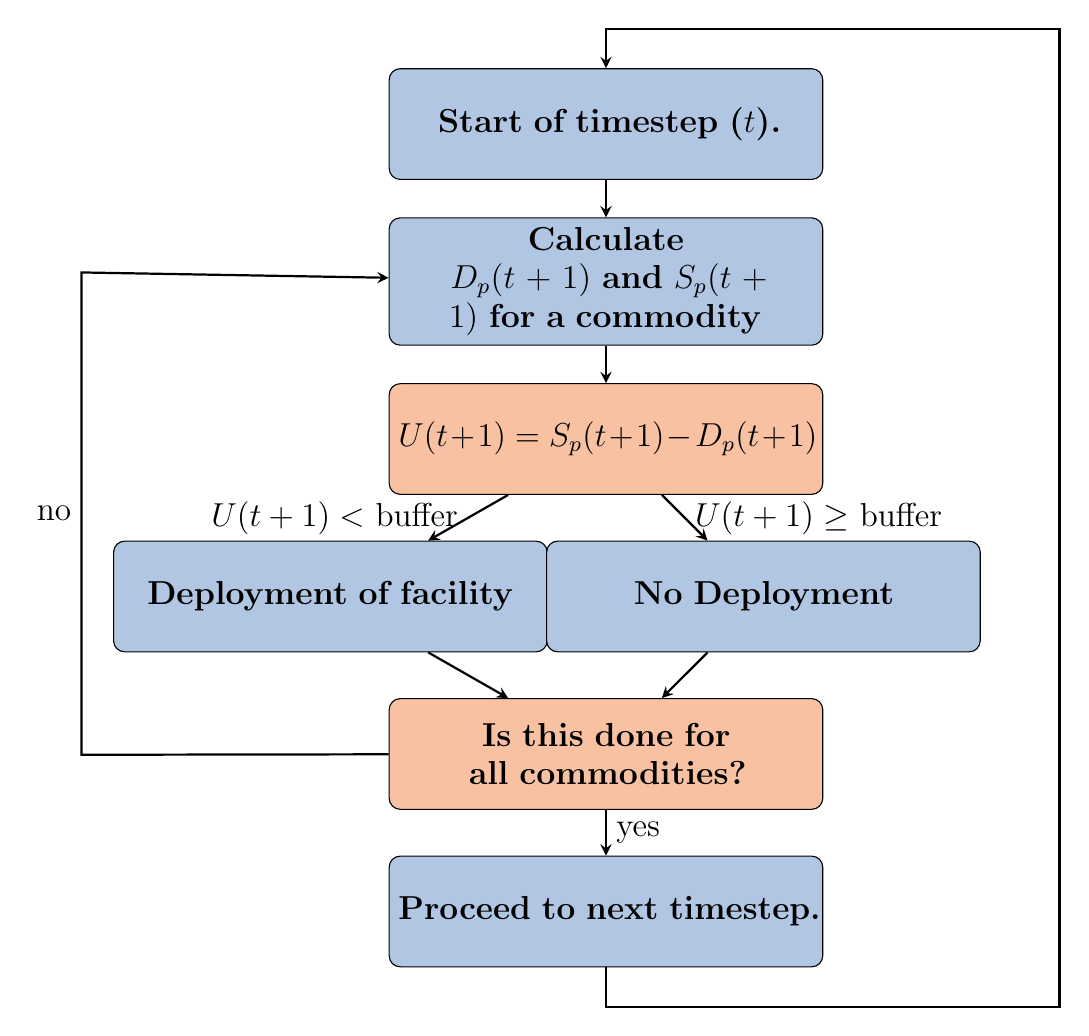
\begin{tikzpicture}[node distance=2cm]
	\tikzstyle{every node}=[font=\large]
	\node (Start) [bblock] {\textbf{Start of timestep ($t$).}};
	\node (Predict) [bblock, below of=Start] {\textbf{Calculate \\ $D_p(t+1)$ and $S_p(t+1)$ for a commodity}};
	\node (IsThere) [oblock, below of=Predict]{\textbf{$U(t+1) = S_p(t+1)-D_p(t+1)$}};
	\node (Deploy) [bblock, below of=IsThere, xshift = -3.5cm]{\textbf{Deployment of facility}};
	\node (NoDeploy) [bblock, right of=Deploy, xshift = 3.5cm]{\textbf{No Deployment} };
	\node (All) [oblock, below of=Deploy, xshift = 3.5cm] {\textbf{Is this done for all commodities?}};
	\node (End) [bblock, below of=All] {\textbf{Proceed to next timestep.}};
	
	\draw [arrow] (Start) -- (Predict); 
	\draw [arrow] (Predict) -- (IsThere);
	\draw [arrow] (IsThere) -- node[anchor=east] {$U(t+1) <$ buffer} (Deploy);
	\draw [arrow] (IsThere) -- node[anchor=west] {$U(t+1) \geq$ buffer} (NoDeploy);
	\draw [arrow] (Deploy) -- (All);
	\draw [arrow] (NoDeploy) -- (All);
	\draw [arrow] (All) -- node[anchor=west] {yes} (End);
	\draw [arrow] (All) -- ([shift={(-3.9cm,0.7cm)}]All.south west)-- node[anchor=east] {no} ([shift={(-3.9cm,-0.7cm)}]Predict.north west)--(Predict);
	\draw [arrow] (End) |-([shift={(3cm,-0.5cm)}]End.south east)-- ([shift={(3cm,0.5cm)}]Start.north east)-|(Start);
	\end{tikzpicture}
}
\caption{\deploy logic flow at every timestep in \Cyclus \cite{chee_demonstration_2019}.}
\label{fig:flow}
\end{figure}
\column[t]{5cm}
\vspace{2cm}
\\
$D_p : Predicted Demand$ \\
$S_p : Predicted Supply$ \\
$U = S_p-D_p$
\end{columns}
\end{frame}

\begin{frame}
\frametitle{\deploy Prediction Methods}
Non-Optimizing Methods 
\begin{itemize}
\item Moving Average (\texttt{ma})
\item Autoregressive Moving Average (\texttt{arma})
\item Autoregressive Heteroskedasticity (\texttt{arch})
\end{itemize}
Deterministic-Optimizing Methods 
\begin{itemize}
\item Fast Fourier Transform (\texttt{fft})
\item Polynomial Fit (\texttt{poly})
\item Exponential Smoothing
\item Triple Exponential Smoothing (\texttt{holt-winters})
\end{itemize}
Stochastic-Optimizing Methods 
\begin{itemize}
\item Auto-Regressive Integrated Moving Averages (\texttt{ARIMA})
\end{itemize}
\end{frame}

\begin{frame}
\frametitle{Breakdown of Results}
4 transition scenarios sought to minimize undersupply and under capacity of 
all commodities.
\begin{enumerate}
	\item EG01-23 ($P(t) = P_0$)
	\item EG01-24 ($P(t) = P_0 + rt$)
	\item EG01-29 ($P(t) = P_0)$
	\item EG01-30 ($P(t) = P_0 + rt$)
\end{enumerate}

This is achieved by:
\begin{enumerate}
	\item Comparison of prediction methods for each of 4 scenarios is conducted 
	to determine the best method. 
	\item Sensitivity analysis of power supply buffer is conducted to determine 
	best buffer size. 
	\item Using best prediction method, look ahead rate, buffer size, demonstrate \deploy 
	deploying reactor and supporting facilities to meet power demand 
	for 4 scenarios. 
\end{enumerate}

\end{frame}

\begin{frame}
\frametitle{Comparison of Prediction Methods}
\textbf{EG01-23 Constant Power Demand Transition Scenario}

\begin{figure}[htbp!]
	\begin{center}
		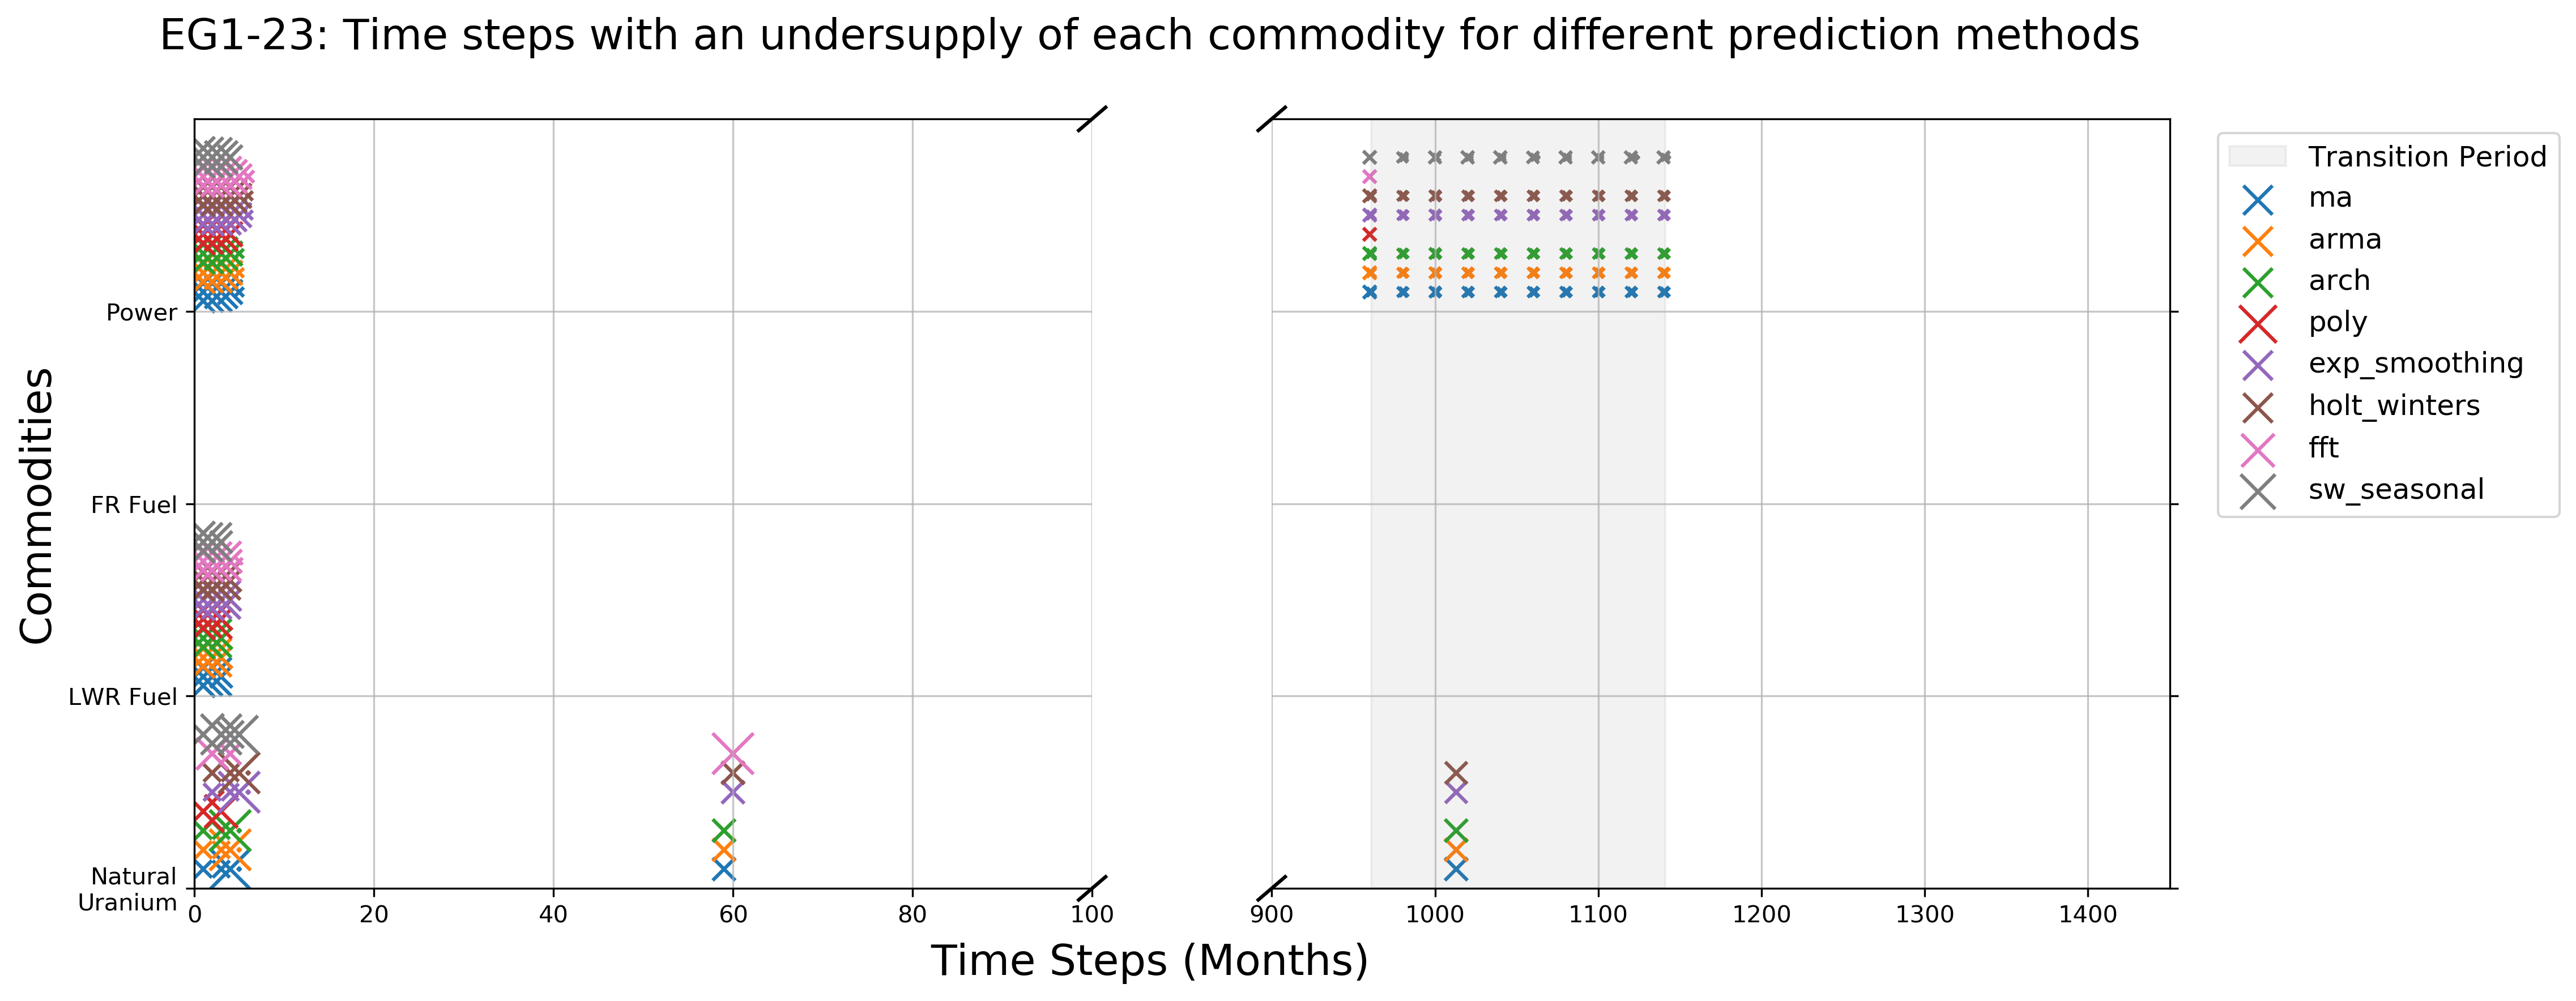
\includegraphics[width=\textwidth]{images/eg23-undersupply.png}
	\end{center}
	\caption{Time dependent undersupply of commodities for different
		prediction methods for the EG01-23 Transition Scenario with Constant Power Demand. The
		size of each cross is based on the size of the undersupply.
		Fewer crosses on plot indicates the method is more successful at preventing undersupply 
		of each commodity}
\end{figure}
\end{frame}

\begin{frame}
\frametitle{Comparison of Prediction Methods}
\textbf{EG01-23 Constant Power Demand Transition Scenario}
\begin{figure}[htbp!]
\begin{center}
	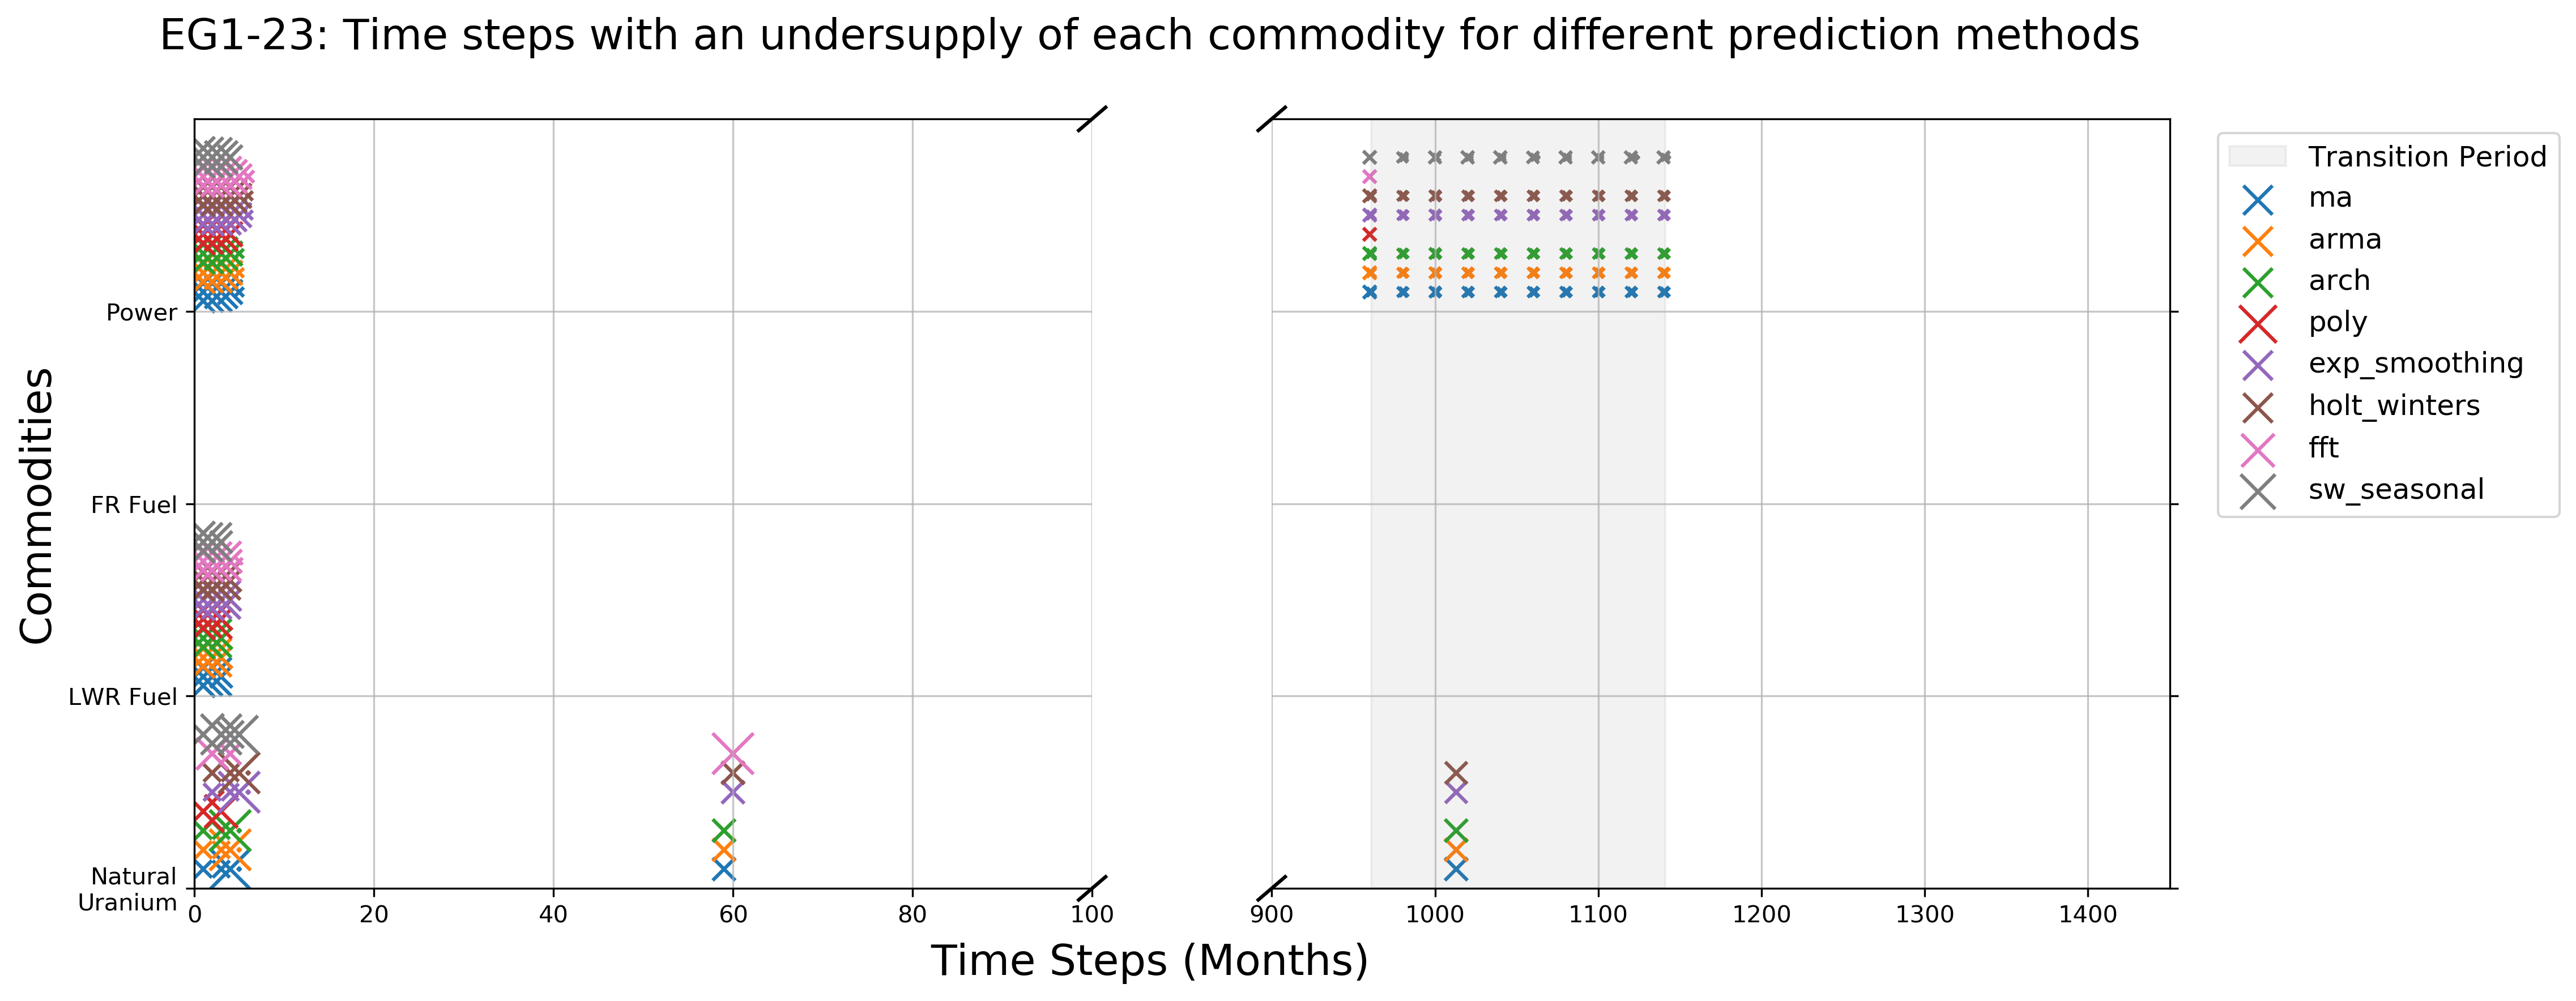
\includegraphics[width=\textwidth]{images/eg23-undersupply.png}
\end{center}
\caption{Time dependent undersupply of commodities for different
	prediction methods for the EG01-23 Transition Scenario with Constant Power Demand. The
	size of each cross is based on the size of the undersupply.
	Fewer crosses on plot indicates the method is more successful at preventing under capacity 
	of each commodity}
\end{figure}
\end{frame}

\begin{frame}
\frametitle{Best Performing Transition Scenarios}
\textbf{Undersupply and under capacity of commodities for the best performing transition scenarios} 
\begin{table}[]
\centering
\caption{Undersupply/capacity of commodities for the best performing EG01-EG23,24,29,30 transition scenarios.}
\label{tab:all-power}
\footnotesize
\begin{tabularx}{\textwidth}{l|RRRR}
\hline
& \multicolumn{3}{|c}{\textbf{Undersupplied Time Steps}} \\ \hline
\textbf{Transition Scenario} & EG01-EG23 & 
EG01-EG24 & EG01-EG29 & 
EG01-EG30 \\ 
\textbf{Power Demand} &Constant&Linearly Increasing&Constant&Linearly Increasing \\
\textbf{Prediction Method} &\texttt{poly}&\texttt{fft}&\texttt{poly}& \texttt{fft}\\
\textbf{Power Supply Buffer [MW]} &0&6000&0&8000 \\ \hline
\textbf{Commodities} \\ 
Natural Uranium		    & 2 	& 3  &  1  & 1 \\ 
\gls{LWR} Fuel     	    & 4 	& 6  &  1  & 2\\ 
\gls{SFR} Fuel     	    &  0 	& 0  &  2  & 2\\ 
\gls{MOX} \gls{LWR} Fuel &-&-&2&2 \\
Power      				&  6 	& 7  &  4 &  5\\ 
\gls{LWR} Spent Fuel	& 1 	& 1  & 1 & 1\\ 
\gls{SFR} Spent Fuel     	    &  1 	& 1  &  1  & 1\\ 
\gls{MOX} \gls{LWR} Spent Fuel &-&-&1&1 \\ \hline 
\end{tabularx}
\end{table}

\end{frame}

\begin{frame}
\frametitle{Conclusion}
These results demonstrate that by carefully selecting \deploy 
parameters, we are able to \textbf{effectively automate deployment}
of reactor and supporting facilities to set up 
constant and linearly increasing power demand transition scenarios
for EG01-23, EG01-24, EG01-29, and EG01-30 with minimal 
power undersupply. 
\vspace{1em}
\\
Not completely eliminating undersupply and under capacity of 
commodities in the simulation is expected 
since without time series data 
at the beginning of the simulation, \deploy takes a few 
time steps to collect time series data about power demand 
to predict and start deploying reactor and supporting 
fuel cycle facilities. 

\end{frame}
\section{Depletion and UDB}
\input{teddy}
\section{SaltProc}
\begin{frame}
\frametitle{SaltProc flowchart}
\vspace{-2mm}
\begin{figure}[ht!] % replace 't' with 'b' to \centering
	\centering
	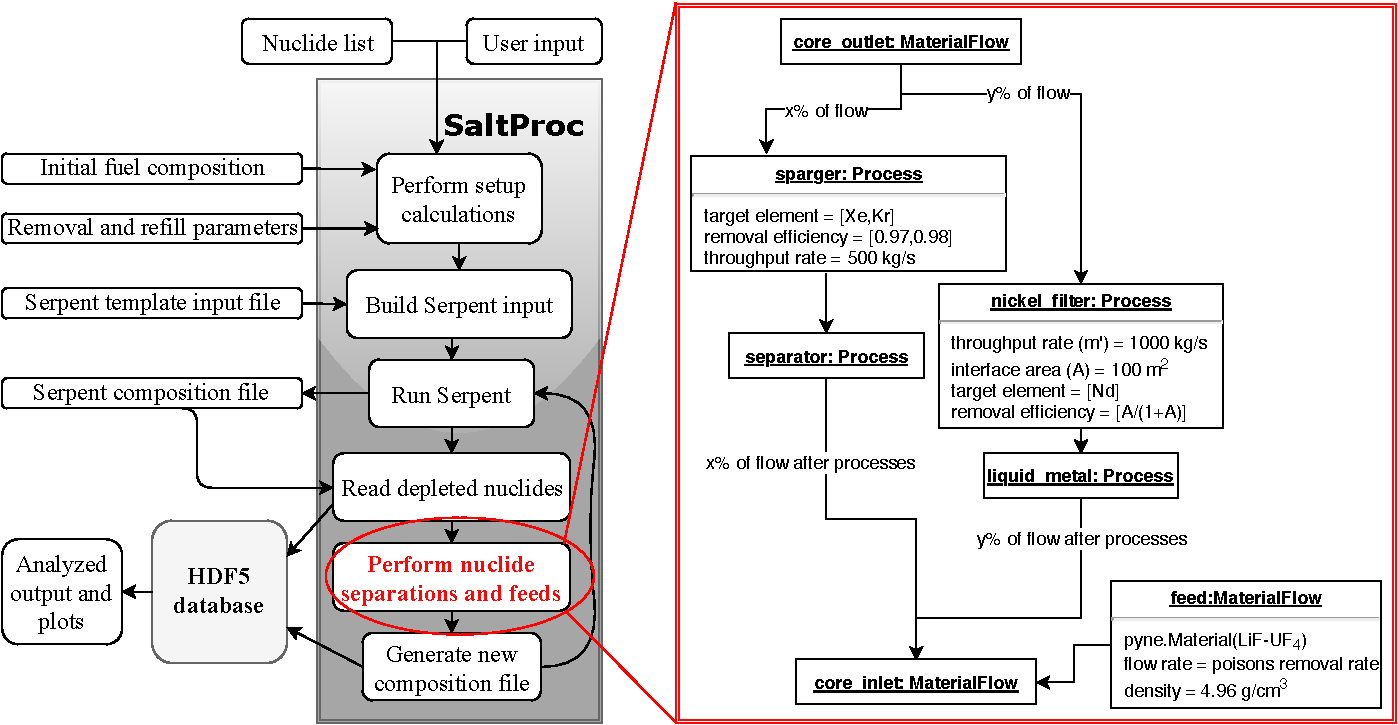
\includegraphics[width=1.05\textwidth]{./images/saltproc_flowchart.pdf}
	\caption{Tentative generic flowchart for SaltProc v1.0 python package.}
\end{figure}

\end{frame}

\section{Acknowledgments}
\begin{frame}
\frametitle{Acknowledgement}
This work is supported by U.S. Department of Energy, 
Nuclear Energy University Program, under contract 
\#NEUP-FY16-10512. 
\end{frame}


%%--------------------------------%%
%%--------------------------------%%
\begin{frame}[allowframebreaks]
  \frametitle{References}
  \bibliographystyle{plain}
  {\footnotesize \bibliography{2019-09-05-group.bib} }
\end{frame}

%%--------------------------------%%

\end{document}

